\section{存在、唯一与稳定性}
\label{sec:ellip-wellposed}

弱形式只是把问题重新写了一遍，解是否存在、是否唯一、是否连续依赖于数据，都还不知道。上一节的三种弱形式有共同的结构：在Hilbert空间$H$中求$u$，使得对所有$v\in H$有$a(u,v)=\ell(v)$。把这个抽象问题解决一次，再逐个边界条件检验假设。

\subsection{Lax--Milgram方法}
\label{sec:ellip-lax-milgram}

先看有限维。考虑方程组$\bm{A}\bm{x}=\bm{b}$，设存在$\alpha>0$，对所有$\bm{x}$有
\[
 \bm{x}^\top\bm{A}\bm{x}\geq\alpha\lVert\bm{x}\rVert_2^2 .
\]
这时矩阵一定可逆，因为$\bm{A}\bm{x}=\bm{0}$推出$\alpha\lVert\bm{x}\rVert_2^2\leq0$。这里不要求$\bm{A}$对称。

下面用一个非对称的矩阵核对：
\[
 \bm{A}=\begin{pmatrix}2&1\\-1&2\end{pmatrix},\qquad\bm{b}=\begin{pmatrix}3\\1\end{pmatrix}.
\]
二次型里的反对称部分互相抵消，$\bm{x}^\top\bm{A}\bm{x}=2\lVert\bm{x}\rVert_2^2$，所以$\alpha=2$。方程的解是$\bm{x}=(1,1)^\top$，并且
\[
 \lVert\bm{x}\rVert_2=\sqrt2\approx1.41\leq\frac{\lVert\bm{b}\rVert_2}{\alpha}=\frac{\sqrt{10}}2\approx1.58 .
\]

这个下界同时给出了可逆性和解的大小，无限维只需把三件事分别补上：把$a$变成算子，由下界得到单射与闭值域，再说明值域没有缺失的方向。第一件事要用Riesz表示定理：Hilbert空间上的每个有界线性泛函都能写成与唯一向量的内积，可参考\BookChapterRef{chap:linear-functionals}{卷四第16章“线性泛函”}。需要的条件如下。

\begin{definition}[有界与强制]
\label{def:ellip-bounded-coercive}
设$H$是实Hilbert空间，$a:H\times H\to\mathbb{R}$是双线性型。若存在$M>0$使
\begin{equation}
 \lvert a(u,v)\rvert\leq M\lVert u\rVert_H\lVert v\rVert_H\qquad\text{对所有}\ u,v\in H,
 \label{eq:ellip-bounded}
\end{equation}
就称$a$有界。若存在$\alpha>0$使
\begin{equation}
 a(v,v)\geq\alpha\lVert v\rVert_H^2\qquad\text{对所有}\ v\in H,
 \label{eq:ellip-coercive}
\end{equation}
就称$a$具有\term{强制性}（coercivity）。
\end{definition}

\begin{theorem}[Lax--Milgram定理]
\label{thm:ellip-lax-milgram}
设$H$是实Hilbert空间，$a$是$H$上有界且强制的双线性型，$\ell\in H^*$。则存在唯一的$u\in H$，使
\begin{equation}
 a(u,v)=\ell(v)\qquad\text{对所有}\ v\in H,
 \label{eq:ellip-abstract}
\end{equation}
并且
\begin{equation}
 \lVert u\rVert_H\leq\frac{\lVert\ell\rVert_{H^*}}{\alpha}.
 \label{eq:ellip-lm-estimate}
\end{equation}
\end{theorem}

\begin{proof}
\emph{第一步，化为算子方程。}由Riesz表示定理，对固定的$u$，$v\mapsto a(u,v)$是有界线性泛函，所以存在唯一的$Tu\in H$，使
\[
 a(u,v)=\langle Tu,v\rangle\qquad\text{对所有}\ v\in H .
\]
同样存在$h\in H$，使$\ell(v)=\langle h,v\rangle$，且$\lVert h\rVert_H=\lVert\ell\rVert_{H^*}$。由$a$的双线性，$T$线性。取$v=Tu$，式~\eqref{eq:ellip-bounded}给出$\lVert Tu\rVert_H\leq M\lVert u\rVert_H$，所以$T$有界。式~\eqref{eq:ellip-abstract}等价于$Tu=h$。

\emph{第二步，下界。}由强制性和Cauchy--Schwarz不等式，
\[
 \alpha\lVert v\rVert_H^2\leq a(v,v)=\langle Tv,v\rangle\leq\lVert Tv\rVert_H\lVert v\rVert_H .
\]
于是
\[
 \lVert Tv\rVert_H\geq\alpha\lVert v\rVert_H\qquad\text{对所有}\ v\in H .
\]
这说明$T$是单射。

\emph{第三步，值域闭。}设$Tv_n\to y$。对差$v_n-v_m$用下界，得到
\[
 \lVert v_n-v_m\rVert_H\leq\frac1\alpha\lVert Tv_n-Tv_m\rVert_H ,
\]
所以$(v_n)$是Cauchy列，收敛到某个$v$。$T$连续，得到$Tv=y$，所以$y$在值域中。

\emph{第四步，值域是全空间。}闭子空间的正交补为零时，子空间就是全空间。设$z$与值域正交。特别地，$z\perp Tz$，于是
\[
 \alpha\lVert z\rVert_H^2\leq a(z,z)=\langle Tz,z\rangle=0 ,
\]
所以$z=0$。因此$T$是双射，$u=T^{-1}h$是唯一的解。

\emph{第五步，估计。}在下界中取$v=u$，得到
\[
 \alpha\lVert u\rVert_H\leq\lVert Tu\rVert_H=\lVert h\rVert_H=\lVert\ell\rVert_{H^*} .
\]
\end{proof}

图~\ref{fig:ellip-lax-milgram}把第三、四步画了出来。下界保证蓝色的值域是闭的，不会缺少极限点；强制性保证与值域垂直的方向$z$不存在，因为若有这样的$z$，$Tz$也在值域中，与$z$垂直，就意味着$a(z,z)=0$。

\begin{BookInlineFigure}
  \centering
  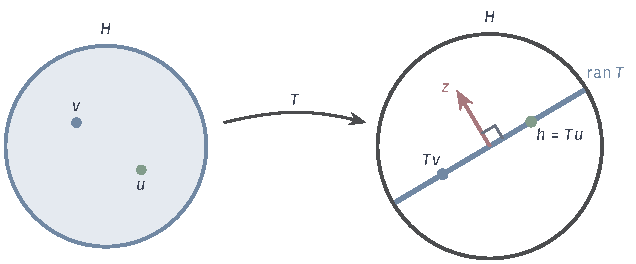
\includegraphics[width=108mm]{figures/06-differential-equations/02-partial-differential-equations/tikz/ellip-lax-milgram/figure.pdf}
  \caption{Lax--Milgram定理证明的几何图景。Riesz表示把$a$变成算子$T$，把$\ell$变成向量$h$，弱问题化为$Tu=h$。下界$\lVert Tv\rVert_H\geq\alpha\lVert v\rVert_H$使值域$\operatorname{ran}T$（蓝线）是闭子空间；红色的$z$若垂直于值域，强制性推出$z=0$，所以值域就是全空间。}
  \label{fig:ellip-lax-milgram}
\end{BookInlineFigure}

\paragraph{各条件的作用}
由式~\eqref{eq:ellip-lm-estimate}，数据之差$\ell_1-\ell_2$导致的解之差满足
\begin{equation}
 \lVert u_1-u_2\rVert_H\leq\frac{\lVert\ell_1-\ell_2\rVert_{H^*}}{\alpha}.
 \label{eq:ellip-lm-stability}
\end{equation}
所以弱问题适定：解存在、唯一，且连续依赖于右端。强制常数$\alpha$越小，同样的数据扰动带来的解的变化可能越大。

三个条件的分工很清楚。有界性让$T$有定义，而且是连续的。强制性同时负责单射、闭值域和满射。$\ell\in H^*$让右端能被表示成向量。

强制性是充分条件，不是必要条件。旋转矩阵$\begin{pmatrix}0&1\\-1&0\end{pmatrix}$可逆，却有$\bm{x}^\top\bm{A}\bm{x}=0$，定理不能用，但这只说明这条路走不通。而在具体方程中，强制性失败时往往确实出了问题：下面的Neumann问题就是这样。

$\ell$有界也不能省略。在$d=2$的单位圆盘上取点源，$\Phi$的梯度大小是$1/(2\pi r)$，能量积分
\[
 \int_{\lVert\bm{x}\rVert_2<1}\lVert\nabla\Phi\rVert_2^2\,\mathrm{d}\bm{x}=\int_0^1\frac{2\pi r}{4\pi^2r^2}\,\mathrm{d}r
\]
对数发散，所以点源问题的解不在$H^1$中。这与“点值不是$H^1_0$上的有界泛函”是同一件事的两面。

\subsection{Dirichlet问题}
\label{sec:ellip-dirichlet}

取$H=H^1_0(\Omega)$。式~\eqref{eq:ellip-uniform}的第二个条件和Cauchy--Schwarz不等式给出有界性：
\[
 \lvert a(u,v)\rvert\leq\kappa_{\max}\lVert\nabla u\rVert_2\lVert\nabla v\rVert_2 .
\]
强制性则要比较$\lVert\nabla v\rVert_2$与$\lVert v\rVert_{H^1}$。式~\eqref{eq:ellip-gradient-control}只控制了梯度，还需要用梯度控制函数本身。

这里需要的工具是Poincaré不等式，由卷四的结论，若$\Omega$有界，存在常数$C_P$，使
\begin{equation}
 \lVert v\rVert_2\leq C_P\lVert\nabla v\rVert_2\qquad\text{对所有}\ v\in H^1_0(\Omega).
 \label{eq:ellip-poincare}
\end{equation}
在$(0,1)$上最优常数是$1/\pi$，它在最低特征函数$\sin(\pi x)$上取到。这个不等式的含义是：函数在边界上被钉在零，要长高就必须爬坡，高度被坡度限制。

由式~\eqref{eq:ellip-poincare}，$\lVert\nabla v\rVert_2$在$H^1_0(\Omega)$上是与$H^1$范数等价的范数，因为
\[
 \lVert\nabla v\rVert_2^2\leq\lVert v\rVert_{H^1}^2\leq(1+C_P^2)\lVert\nabla v\rVert_2^2 .
\]
下面在$H^1_0(\Omega)$上取$\lVert v\rVert_{H^1_0}=\lVert\nabla v\rVert_2$，这时$\alpha=\kappa_{\min}$，$M=\kappa_{\max}$。

\begin{theorem}[Dirichlet问题的适定性]
\label{thm:ellip-dirichlet}
设$\Omega$是有界开集，$\bm{A}$一致椭圆，$f\in L^2(\Omega)$。则$-\nabla\cdot(\bm{A}\nabla u)=f$、零Dirichlet边界的弱解$u\in H^1_0(\Omega)$存在唯一，且
\begin{equation}
 \lVert\nabla u\rVert_2\leq\frac{C_P}{\kappa_{\min}}\lVert f\rVert_2 .
 \label{eq:ellip-dirichlet-estimate}
\end{equation}
若$\Omega$是有界Lipschitz区域，边界值$g=\operatorname{Tr}R$，$R\in H^1(\Omega)$，弱解同样存在唯一，且
\begin{equation}
 \lVert\nabla u\rVert_2\leq\frac{C_P}{\kappa_{\min}}\lVert f\rVert_2+\Bigl(1+\frac{\kappa_{\max}}{\kappa_{\min}}\Bigr)\lVert\nabla R\rVert_2 .
 \label{eq:ellip-dirichlet-inhom}
\end{equation}
\end{theorem}

\begin{proof}
先看$g=0$。令$\ell(v)=\int_\Omega fv\,\mathrm{d}\bm{x}$。由Cauchy--Schwarz不等式和式~\eqref{eq:ellip-poincare}，
\[
 \lvert\ell(v)\rvert\leq\lVert f\rVert_2\lVert v\rVert_2\leq C_P\lVert f\rVert_2\lVert\nabla v\rVert_2 ,
\]
所以$\lVert\ell\rVert\leq C_P\lVert f\rVert_2$。定理~\ref{thm:ellip-lax-milgram}给出唯一的解和估计式~\eqref{eq:ellip-dirichlet-estimate}。

再看一般的$g$。令$u=R+w$，$w$满足式~\eqref{eq:ellip-lifted}。其右端泛函满足
\[
 \Bigl\lvert\int_\Omega fv\,\mathrm{d}\bm{x}-a(R,v)\Bigr\rvert\leq\bigl(C_P\lVert f\rVert_2+\kappa_{\max}\lVert\nabla R\rVert_2\bigr)\lVert\nabla v\rVert_2 .
\]

定理~\ref{thm:ellip-lax-milgram}给出唯一的$w\in H^1_0(\Omega)$，且$\lVert\nabla w\rVert_2$不超过上式括号内的量除以$\kappa_{\min}$。对$u=R+w$用三角不等式，就得到式~\eqref{eq:ellip-dirichlet-inhom}。

唯一性：若$u_1,u_2$都是弱解，差$u_1-u_2\in H^1_0(\Omega)$满足齐次问题，由已证部分为零。
\end{proof}

式~\eqref{eq:ellip-dirichlet-inhom}说明解的大小由源项和边界提升共同决定，并且提升可以取$H^1$范数最小的那一个，于是估计实际上是对边界数据本身的。

用贯穿的例子核对。$\Omega=(0,1)$，$\kappa_{\min}=1$，$C_P=1/\pi$，$f=1$，$\lVert f\rVert_2=1$。解$u=x(1-x)/2$的导数是$1/2-x$，
\[
 \lVert u'\rVert_2=\Bigl(\int_0^1\bigl(\tfrac12-x\bigr)^2\,\mathrm{d}x\Bigr)^{1/2}=\frac1{\sqrt{12}}\approx0.289,
\]
而估计的上界是$1/\pi\approx0.318$，上界成立且相当紧。若取$f=\sin(\pi x)$，解是$\sin(\pi x)/\pi^2$，此时$\lVert u'\rVert_2=\lVert f\rVert_2/\pi$，估计取到等号，这说明常数$C_P/\kappa_{\min}$不能改进。

\paragraph{解算子与特征基}
第~\ref{sec:ellip-spectral}小节留下了一个问题：一般有界区域上，特征函数组成的基存在吗？弱解理论现在可以回答。设$\bm{A}$对称。定义解算子$S:L^2(\Omega)\to L^2(\Omega)$，$Sf$是源项为$f$的弱解。

由式~\eqref{eq:ellip-dirichlet-estimate}，$S$把$L^2$的有界集映为$H^1_0(\Omega)$的有界集。把$H^1_0(\Omega)$的函数零延拓到一个包含$\Omega$的球上，$H^1$有界集到$L^2$的紧嵌入就给出$S$是紧算子。一维时这一紧性更直接：$H^1(a,b)$的有界集由Sobolev不等式一致有界、等度Hölder连续，由Arzelà--Ascoli定理在$C[a,b]$中相对紧，从而在$L^2(a,b)$中相对紧。

$S$还是自伴的。记$u=Sf$，$w=Sh$，把它们互相作为测试函数，由弱形式和$a$的对称性，
\[
 \langle h,Sf\rangle=a(w,u)=a(u,w)=\langle f,Sh\rangle .
\]
$S$也是正的，且是单射，因为$f\neq0$时$u\neq0$，从而$\langle f,Sf\rangle=a(u,u)>0$。

由紧自伴算子的谱定理（可参考\BookChapterRef{chap:operator-spectra}{卷四第18章“算子谱”}），存在$L^2(\Omega)$的标准正交基$(e_k)$，使$Se_k=\mu_ke_k$，$\mu_k>0$，$\mu_k\to0$。令$\lambda_k=1/\mu_k$，则$\lambda_k\to\infty$，$e_k\in H^1_0(\Omega)$，且
\[
 a(e_k,v)=\lambda_k\langle e_k,v\rangle\qquad\text{对所有}\ v\in H^1_0(\Omega) .
\]
这就是特征问题~\eqref{eq:ellip-eigenproblem}的弱形式，而$Sf=\sum_k\mu_kf_ke_k$正是式~\eqref{eq:ellip-spectral-solution}。

\subsection{Neumann问题}
\label{sec:ellip-neumann}

在式~\eqref{eq:ellip-weak-neumann}中取$v=1$，$\nabla v=0$，左端为零，得到
\begin{equation}
 \int_\Omega f\,\mathrm{d}\bm{x}+\int_{\partial\Omega}g\,\mathrm{d}S=0.
 \label{eq:ellip-neumann-compat}
\end{equation}
这是相容条件~\eqref{eq:ellip-interval-compat}的多维形式，意义仍是总量收支为零。不满足这个条件，弱解就不存在。

反过来，$a$在$H^1(\Omega)$上不强制：常数函数$v=1$满足$a(v,v)=0$。若$\Omega$连通，$a(v,v)=0$蕴含$\nabla v=0$，$v$是常数，所以核空间恰好是常数。若$\Omega$不连通，每个连通分支上都可以独立取常数，核空间更大，相容条件也要逐分支成立。

这与奇异矩阵的情形完全相同。图~\ref{fig:ellip-energy-valley}用两个未知量的二次函数$\frac12\bm{c}^\top\bm{K}\bm{c}-\bm{b}^\top\bm{c}$比较三种情形，其极小点满足$\bm{K}\bm{c}=\bm{b}$。(a)是正定的$\bm{K}$，等高线是椭圆，有唯一的极小点。(b)的$\bm{K}=\begin{pmatrix}1&-1\\-1&1\end{pmatrix}$有核方向$(1,1)^\top$，$\bm{b}$与核方向正交时，极小点组成一条线。(c)的$\bm{b}$不与核方向正交，函数沿核方向一直下降，没有极小点。

\begin{BookInlineFigure}
  \centering
  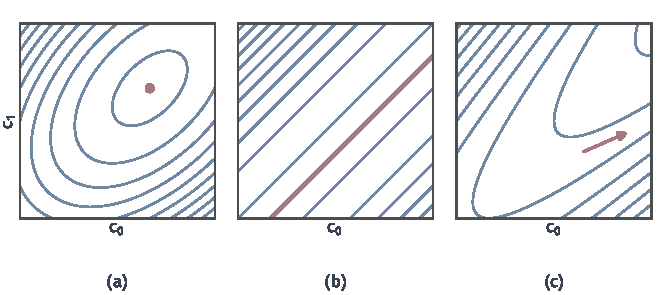
\includegraphics[width=112mm]{figures/06-differential-equations/02-partial-differential-equations/matplotlib/ellip-energy-valley/figure.pdf}
  \caption{核空间的有限维图景，蓝线是$\frac12\bm{c}^\top\bm{K}\bm{c}-\bm{b}^\top\bm{c}$的等高线。(a)$\bm{K}$的对角元为$2$、非对角元为$-1$，$\bm{b}=(1,1)^\top$，唯一极小点$(1,1)$（红）。(b)$\bm{K}$奇异，$\bm{b}=(1,-1)^\top$与核方向$(1,1)^\top$正交，极小点是红线$c_0-c_1=1$。(c)同样的$\bm{K}$，$\bm{b}=(1,0)^\top$，沿红色箭头方向函数无下界。}
  \label{fig:ellip-energy-valley}
\end{BookInlineFigure}

处理办法是先去掉核方向。取零均值子空间
\begin{equation}
 V=\Bigl\{v\in H^1(\Omega):\int_\Omega v\,\mathrm{d}\bm{x}=0\Bigr\}.
 \label{eq:ellip-zero-mean}
\end{equation}
由卷四的零均值Poincaré不等式，在有界连通Lipschitz区域上存在$C_W$，使$\lVert v\rVert_2\leq C_W\lVert\nabla v\rVert_2$对$v\in V$成立。于是$\lVert\nabla\cdot\rVert_2$是$V$上的等价范数，$a$在$V$上强制，$\alpha=\kappa_{\min}$。

迹算子有界，再用上面的等价范数，就存在常数$C_\partial$，使
\begin{equation}
 \lVert\operatorname{Tr}v\rVert_{L^2(\partial\Omega)}\leq C_\partial\lVert\nabla v\rVert_2\qquad\text{对所有}\ v\in V.
 \label{eq:ellip-trace-zero-mean}
\end{equation}

\begin{theorem}[Neumann问题的适定性]
\label{thm:ellip-neumann}
设$\Omega$是有界连通Lipschitz区域，$\bm{A}$一致椭圆，$f\in L^2(\Omega)$，$g\in L^2(\partial\Omega)$。式~\eqref{eq:ellip-weak-neumann}有解当且仅当式~\eqref{eq:ellip-neumann-compat}成立。此时解在相差一个常数的意义下唯一，零均值的解$u\in V$满足
\begin{equation}
 \lVert\nabla u\rVert_2\leq\frac1{\kappa_{\min}}\bigl(C_W\lVert f\rVert_2+C_\partial\lVert g\rVert_{L^2(\partial\Omega)}\bigr).
 \label{eq:ellip-neumann-estimate}
\end{equation}
\end{theorem}

\begin{proof}
必要性已经证明。设相容条件成立，令$\ell(v)=\int_\Omega fv+\int_{\partial\Omega}gv$。在$V$上，由Cauchy--Schwarz不等式和式~\eqref{eq:ellip-trace-zero-mean}，
\[
 \lvert\ell(v)\rvert\leq\bigl(C_W\lVert f\rVert_2+C_\partial\lVert g\rVert_{L^2(\partial\Omega)}\bigr)\lVert\nabla v\rVert_2 .
\]
定理~\ref{thm:ellip-lax-milgram}给出唯一的$u\in V$和估计式~\eqref{eq:ellip-neumann-estimate}，它对所有$v\in V$满足$a(u,v)=\ell(v)$。

还要把测试函数从$V$扩大到$H^1(\Omega)$。任取$v\in H^1(\Omega)$，令$\bar v=\lvert\Omega\rvert^{-1}\int_\Omega v$，则$v-\bar v\in V$。$a(u,\bar v)=0$，因为常数的梯度为零；$\ell(\bar v)=0$，因为相容条件成立。于是
\[
 a(u,v)=a(u,v-\bar v)=\ell(v-\bar v)=\ell(v) .
\]

若$u_1,u_2$都是解，差$z=u_1-u_2$满足$a(z,z)=0$，由式~\eqref{eq:ellip-gradient-control}，$\nabla z=0$，$\Omega$连通，故$z$是常数。
\end{proof}

用前面的例子核对。$\Omega=(0,1)$，$f=1-2x$，$C_W=1/\pi$，$\lVert f\rVert_2=1/\sqrt3$。解的导数$u'=x^2-x$，
\[
 \lVert u'\rVert_2=\Bigl(\int_0^1(x^2-x)^2\,\mathrm{d}x\Bigr)^{1/2}=\frac1{\sqrt{30}}\approx0.183,
\]
上界$C_W\lVert f\rVert_2=1/(\pi\sqrt3)\approx0.184$，几乎取到等号，因为$f$很接近第一个非常数的特征函数。

这里的估计式~\eqref{eq:ellip-neumann-estimate}只对零均值的代表成立，也只能如此：加上常数后，解可以任意大，却仍是解。

\subsection{Robin问题}
\label{sec:ellip-robin}

Robin问题的$a_\beta$比$a$多了边界项$\int_{\partial\Omega}\beta v^2$。常数函数在$a$中的能量为零，在这里要付出边界代价。边界项能否像Poincaré不等式那样补足对函数本身的控制？

先看一个可以直接解的例子。在$(0,1)$上取$-u''=1$，两端都是$\bm{n}\cdot\nabla u+\beta u=0$，$\beta>0$。由对称性，解形如$x(1-x)/2+c$，代入左端条件：
\[
 -u'(0)+\beta u(0)=-\frac12+\beta c=0 ,
\]
所以
\begin{equation}
 u(x)=\frac{x(1-x)}2+\frac1{2\beta}.
 \label{eq:ellip-robin-example}
\end{equation}

图~\ref{fig:ellip-robin-beta}显示$\beta$的作用。$\beta\to\infty$时，边界换热无限快，解收敛到Dirichlet问题的解。$\beta\to0$时，$u$的常数部分$1/(2\beta)$趋于无穷，解的范数爆炸；极限的Neumann问题$f=1$本来就不相容。收支也是平衡的：总产热$1$经两端散出，$\beta(u(0)+u(1))=1$。

\begin{BookInlineFigure}
  \centering
  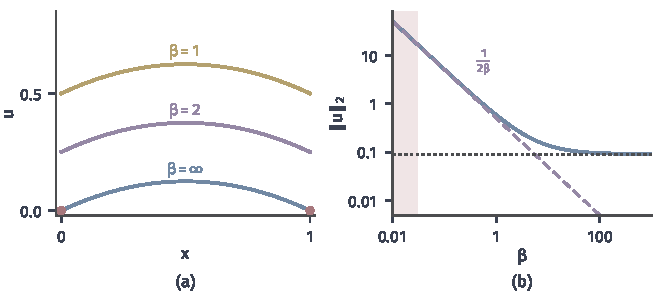
\includegraphics[width=112mm]{figures/06-differential-equations/02-partial-differential-equations/matplotlib/ellip-robin-beta/figure.pdf}
  \caption{$-u''=1$、两端Robin条件的解。(a)$\beta=1,2$时（黄、紫）解被整体抬高$1/(2\beta)$，$\beta\to\infty$时趋于蓝线的Dirichlet解。(b)$\lVert u\rVert_2$随$\beta$的变化：$\beta\to0$时沿紫色虚线$1/(2\beta)$爆炸（红底区域接近不相容的Neumann极限），$\beta\to\infty$时趋于点线$1/\sqrt{120}$。}
  \label{fig:ellip-robin-beta}
\end{BookInlineFigure}

这个例子说明，强制常数必然随$\beta$退化，所以需要一条统一的不等式，把$\beta$的作用写进去。

\begin{lemma}[边界项给出的Poincaré不等式]
\label{lem:ellip-robin-poincare}
设$\Omega$是有界连通Lipschitz区域，$\beta\in L^\infty(\partial\Omega)$，$\beta\geq0$，$\int_{\partial\Omega}\beta\,\mathrm{d}S>0$。则存在常数$C_R$，使
\begin{equation}
 \lVert v\rVert_2^2\leq C_R\Bigl(\lVert\nabla v\rVert_2^2+\int_{\partial\Omega}\beta v^2\,\mathrm{d}S\Bigr)\qquad\text{对所有}\ v\in H^1(\Omega).
 \label{eq:ellip-robin-poincare}
\end{equation}
\end{lemma}

\begin{proof}
用反证法。若不等式不成立，存在序列$(v_n)\subset H^1(\Omega)$，$\lVert v_n\rVert_2=1$，并且
\[
 \lVert\nabla v_n\rVert_2^2+\int_{\partial\Omega}\beta v_n^2\,\mathrm{d}S\to0 .
\]
序列在$H^1$中有界，由$H^1(\Omega)$到$L^2(\Omega)$的紧嵌入，有子列在$L^2(\Omega)$中收敛到某个$v$，$\lVert v\rVert_2=1$。子列的梯度趋于零，所以子列在$H^1$中也是Cauchy列，收敛到$v$，且$\nabla v=0$。

$\Omega$连通，所以$v$等于常数$c$，由$\lVert v\rVert_2=1$知$c\neq0$。迹算子连续，$\operatorname{Tr}v_n\to c$于$L^2(\partial\Omega)$，$\beta$有界，于是
\[
 \int_{\partial\Omega}\beta v_n^2\,\mathrm{d}S\to c^2\int_{\partial\Omega}\beta\,\mathrm{d}S>0 ,
\]
这与假设矛盾。
\end{proof}

这个证明用了紧嵌入，所以常数$C_R$是非构造性的。证明的核心很直白：能让所有控制量都趋于零的只有常数，而边界上正的$\beta$排除了常数。

\begin{theorem}[Robin问题的适定性]
\label{thm:ellip-robin}
设$\Omega$是有界连通Lipschitz区域，$\bm{A}$一致椭圆，$\beta$满足引理~\ref{lem:ellip-robin-poincare}的条件，$f\in L^2(\Omega)$，$g\in L^2(\partial\Omega)$。则式~\eqref{eq:ellip-weak-robin}存在唯一的解$u\in H^1(\Omega)$，且存在只依赖于$\Omega,\bm{A},\beta$的常数$C$，使
\begin{equation}
 \lVert u\rVert_{H^1}\leq C\bigl(\lVert f\rVert_2+\lVert g\rVert_{L^2(\partial\Omega)}\bigr).
 \label{eq:ellip-robin-estimate}
\end{equation}
\end{theorem}

\begin{proof}
由迹定理，存在$C_{\mathrm{Tr}}$，使
\[
 \lVert\operatorname{Tr}v\rVert_{L^2(\partial\Omega)}\leq C_{\mathrm{Tr}}\lVert v\rVert_{H^1} .
\]
于是$a_\beta$有界：
\[
 \lvert a_\beta(u,v)\rvert\leq\bigl(\kappa_{\max}+\lVert\beta\rVert_\infty C_{\mathrm{Tr}}^2\bigr)\lVert u\rVert_{H^1}\lVert v\rVert_{H^1} .
\]
右端泛函也有界，其范数不超过$\lVert f\rVert_2+C_{\mathrm{Tr}}\lVert g\rVert_{L^2(\partial\Omega)}$。

由式~\eqref{eq:ellip-gradient-control}，令$\kappa_0=\min(\kappa_{\min},1)$，
\[
 a_\beta(v,v)\geq\kappa_0\Bigl(\lVert\nabla v\rVert_2^2+\int_{\partial\Omega}\beta v^2\,\mathrm{d}S\Bigr) .
\]
由式~\eqref{eq:ellip-robin-poincare}，
\[
 \lVert v\rVert_{H^1}^2\leq(1+C_R)\Bigl(\lVert\nabla v\rVert_2^2+\int_{\partial\Omega}\beta v^2\,\mathrm{d}S\Bigr) .
\]
所以$a_\beta$强制，$\alpha=\kappa_0/(1+C_R)$。定理~\ref{thm:ellip-lax-milgram}给出结论。
\end{proof}

条件$\int_{\partial\Omega}\beta>0$不能去掉。$\beta\equiv0$时问题退回Neumann问题，核空间是常数，唯一性丢失。条件$\beta\geq0$也不能随意放宽。在$(0,1)$上取两端$\beta=-2$，考察$-u''=0$，函数$u=1-2x$满足
\[
 -u'(0)+\beta u(0)=2-2=0,\qquad u'(1)+\beta u(1)=-2+2=0 ,
\]
这是一个非零的解，所以齐次问题不唯一。负的$\beta$相当于边界不断向棒内放热，且放热量随温度增长，边界项不再贡献能量，而是削弱能量。

三类边界条件的结论可以这样总结：Dirichlet问题靠零迹排除常数，Robin问题靠边界代价排除常数，Neumann问题排除不了常数，只能把常数方向分离出去，并要求数据与之相容。
